\documentclass[pdftex,12pt,a4paper,twoside]{report}

% Aaron Snsowell Thesis Document

\usepackage[lmargin=3cm,rmargin=2cm,tmargin=2cm,bmargin=2cm]{geometry}
\usepackage{setspace}
\usepackage{framed}
\usepackage[usenames,dvipsnames]{xcolor}
\usepackage{framed}
\usepackage{fancybox}
% Used for images
\usepackage[pdftex]{graphicx}
% Used to get nice (r) and (c) symbols
\usepackage{textcomp}
% Used for equations
\usepackage{mathtools}
% Used for headers
\usepackage{fancyhdr}
% Used for referencing sections
\usepackage{nameref}
% Used for nice " and ' quotes
\usepackage{csquotes}

% Set image path
\graphicspath{{./images/}}


% Set spacing and 'graph indentation
\doublespacing
\setlength{\parindent}{1.5cm}


% Horizontal rule command
\newcommand{\HRule}{\rule{\linewidth}{0.5mm}}

% Command to get current section
\makeatletter
\newcommand*{\currentname}{\@currentlabelname}
\makeatother

% Set up headers
\pagestyle{fancy}
\renewcommand{\headrulewidth}{0.1pt}
\renewcommand{\chaptermark}[1]{\markboth{#1}{}}
\renewcommand{\sectionmark}[1]{\markright{#1}{}}

\fancyhead[RO, LE]{}
\fancyhead[LO]{\small Light Field Deblurring for Robotics Applications}
\fancyhead[RE]{\small \leftmark~(\rightmark)}
\fancyfoot[c]{\small \thepage}

\begin{document}

% Title page
\begin{titlepage}

\begin{center}

% Upper part of the page

\includegraphics[width=4cm]{UQ.png}\\[1.5cm]    

\textsc{\Large \bfseries {\Huge T}HE {\Huge U}NIVERSITY OF {\Huge Q}UEENSLAND}\\[2cm]

\textsc{\large \bfseries Bachelor of Engineering Thesis}\\[1.5cm]


\newlength{\mylength}

\setlength{\fboxsep}{1pt}
\setlength{\mylength}{\linewidth}

\addtolength{\mylength}{-1.5\fboxsep}
\addtolength{\mylength}{-1.5\fboxrule}

\doublebox{%
\parbox{\mylength}
{
\begin{center}
\large Light Field De-blurring for Robotics Applications
\end{center}
}
}

		
\textsc{}\\[1.5cm]

% Author and supervisor
\begin{minipage}{0.8\textwidth}
\begin{flushleft} \large
Student Name: \textsc{Aaron Snoswell}\\[0.1cm]
Course Code: METR4901\\[0.1cm]
Supervisor: Dr. Surya P. N. Singh\\[0.1cm]
Submission Date: 16 June 2014\\[0.1cm]
\end{flushleft}
\end{minipage}




\vfill


{\small A thesis submitted in partial fulfillment of the requirements of the\\
Bachelor of Engineering Degree in Mechatronic Engineering\\[1.5cm]}

\textcolor{Gray}
{
{\small  \bfseries UQ Engineering\\[0.5cm]
Faculty of Engineering, Architecture and Information Technology}
}


\end{center}

\end{titlepage}

% Other pages
\begin{abstract}

This thesis discusses two key computer vision problems; the ability to de-blur a motion-blurred light field image, and the ability to use deconvolution de-blurring methods for images with large depth variation.
An equation describing a 3D Point Spread Function is derived, allowing depth-aware deconvolution to be performed on motion-blurred images.
Depth maps from the commercial Lytro light field camera are analysed and a piecewise linear mapping found that gives calibrated depth map measurements.
By combining these two results, a framework for deconvolution de-blurring of a light field image is described, and an experiment designed to verify a simplified test case.
Several motion-blurred scenes are photographed using a Lytro camera and a means for applying depth-aware deconvolution to light field images is demonstrated.
Quantitative results show improved de-blurring performance compared to traditional 2D deconvolution methods.
To our knowledge, this is the first documented application of deconvolution de-blurring to a motion-blurred light field image.

\end{abstract}

\tableofcontents
\newpage

\listoffigures
\newpage

\listoftables
\newpage


\chapter{Introduction}

Here we are introducing things...


\chapter{Background}

\section{Light Field Theory}

%Side Note
%The first practical work using light fields dates back to a photographic technique known as ‘Integral Photography’, developed by Gabriel Lipmann in 1908.
%Lipmann’s technique involved placing an array of lenses over a piece of film.
%The film was then exposed to a scene, encoding 3D information through the lens pattern. 
%By reversing this process (projecting light through the film, then through an identical lens array), the first 3D pictures were created.
%Modern techniques allow Lipmann’s lens arrays to be printed on a surface, creating what is commonly known as ‘holographic pictures’ that morph and change as the viewer’s perspective changes.
%GIVE MORE INFORMATION ON INTEGRAL PHOTOGRAPHY.
%The ability to create a 3D display in this manner (without extra viewing devices such as 3D glasses) is known as auto-stereoscopic imaging.


The light field is a mathematical description of the way light propagates.
Another name for this is the ‘Plenoptic Function', from the Latin ‘plenus’, meaning full, and ‘optic’, meaning light.
The plenoptic function describes every possible configuration a light ray could ever be in, encompassing the three spatial dimensions, two angular dimensions, temporal changes as well as frequency (colour), phase and polarisation changes.
In most computer vision literature the phase and polarisation elements are ignored, leading to a 7-dimensional definition of the plenoptic function;

\begin{equation}
\label{eq:plenoptic_function}
P = P(V_x, V_y, V_z, \theta, \phi, t, \lambda)
\end{equation}

where $V_x$, $V_y$ and $V_z$ are the spatial dimensions, $\theta$ and $\phi$ are the angular dimensions, $t$ is the temporal dimension and $\lambda$ describes the colour of the ray. 

The plenoptic function in this form was first described by Adelson and Bergen in 1991 \cite{adelson1991plenoptic}.
Adelson and Bergen developed a light field theory by asking the fundamental question \enquote{What can be seen?} They stressed that the plenoptic function is the sole visual communication link between physical objects and the eye.
They also suggest that the function of \enquote*{early vision} in biological and artificial organisms is to sample the derivative of this function along various dimensions such as \enquote*{change in colour with x} or \enquote*{change in brightness with time}.
GIVE DETAIL ABOUT SAMPLING PLENOPTIC FUNCTION EXAMPLES FROM ADELSON PAPER.

In modern computer vision literature a number of parameterisations are used to describe the plenoptic function.
These different representations each provide new insights into the information contained in the light field.

LIGHT SLAB DESCRIPTION AND DISCUSSION.

LIGHT TUBE DESCRIPTION AND DISCUSSION.

POLAR AND/OR DUAL PLANE DESCRIPTION AND DISCUSSION?


Traditional cameras generally sample the Light Field along two spatial dimensions (x and y pixel locations) and in the colour dimension (normally with Red, Green and Blue photon collectors), however there are many instances in which sampling more dimensions of the light field would be beneficial. To this end, in 1996 two light field papers were included in the Siggraph conference proceedings; ‘Light Field Rendering’ by Levoy et al. and ‘The Lumigraph’ by Gortler et al [REFERENCES]. Both these papers described independent research into means for capturing more information from the plenoptic function. Importantly, both groups made the observation that, while the full plenoptic function is seven dimensional, for a region of space free of occluding objects, one space dimension can be disregarded, and the 3D structure of the scene still fully recovered. GO INTO MORE DETAIL ABOUT OCCLUSION FREE SPACE SIMPLIFICATION HERE. This approximation is the basis for most modern light field cameras sampling in four dimensions, and paved the way for the creation of the first practical light field cameras.

All physical cameras (or eyes) can only ever observe a small subset (various ‘slices’) of the ambient light field. As an example, consider the human visual system. The human visual system takes several million samples from the angular dimensions, three points from the lambda dimension (roughly corresponding to the frequencies known as ‘Blue’, ‘Green’ and ‘Red’) and only two samples from the Vx dimension (one each for the left and right eyes). In addition to this, the distribution of sample points is not always linear. The cone cells responsible for detecting colour in the human eye are much more populous in the fovetal region near the centre of the eye, while rod cells that operate in low-light conditions are clustered around the outer edges of the retina.

The work done by Gortler and Levoy (et al.) demonstrated it was possible to capture 4D light field information using a traditional camera sensor with some modifications. While there is active research in developing angle-sensitive pixels, modern light field cameras typically encode angular ray information by mapping ray angles to locations on a traditional 2D camera sensor. Thus, regular spatial resolution is directly traded to gain angular resolution.

For example the Lytro light field camera used in this paper has an 11 mega-pixel sensor chip, however a spatial and angular resolution of only 1080x1080 and 10x10 respectively. The trade-off between angular resolution and spatial resolution is unavoidable when using this technique, and the choice of angular and spatial resolutions limit the functions that can be performed with the captured light field. GIVE EXMPLES OF HOW NOT ALL LIGHT FIELDS ARE EQUAL. DISCUSS THE BENEFITS/DRAWBACKS OF THE LYTRO CAMERA CONFIGURATION. 4D light field sampling has also been performed using multiple traditional cameras separated spatially in a grid, or separated temporally.

GO INTO MORE DETAIL ABOUT LYTRO CAMRERA AND BRIEFLY COMPARE LYTRO WITH RAYTRIX AND OTHER LF CAMERAS (STANFORD MULTI CAMERA ARRAY). ALSO DISCUSS SYNTHETIC LIGHT FIELD CREATION AND GIVE EXMAPLES. HIGHLIGHT BENEFITS AND DRAWBACKS OF SYNTHETIC LIGHT FIELDS VS REAL TEST DATA. MENTION THE APPEARANCE OF LIGHT FIELD CAMERAS ON MOBILE PHONES.

Mapping of ray angles to the 2D camera plane is typically done by placing either a lenslet or mirror array, or a cosine pinhole mask within the light ray path. These approaches are functionally equivalent, however each has disadvantages and benefits. A lenslet or mirror array is di cult to machine and requires custom hardware and precision positioning. On the other hand, a pinhole array can be added to some modern cameras with little modification, however blocks a large majority of the incoming light, thus requiring longer exposure times and increasing the likelihood of motion blurring.

2 OR 3 PARAGRAPHS ABOUT LOW RESOLUTION AND LIGHT FIELD SUPER RESOLUTION PAPER.

POSSIBLY 2-3 MORE PARAGRAPHS ABOUT RECENT LIGHT FIELD RESEARCH AND DEVELOPMENTS.

2 SUMMARISING PARAGRAPHS BRINGING ALL OF THIS INFORMATION BACK TO MY THESIS – HIGHLIGHTING WHAT PARTS I’M GOING TO BE USING, WHAT LF SYMBOLS AND CONVENTIONS I’LL BE USING ETC.



\section{Motion Blur Formation}


\begin{equation}
\label{eq:camera_projection}
k
\begin{bmatrix}
x \\
y \\
1 \\
\end{bmatrix}
=
\begin{bmatrix}
\alpha && s && u_0 \\
0 && \beta && v_0 \\
0 && 0 && 1 \\
\end{bmatrix}
\begin{bmatrix}
r_{11} && r_{12} && r_{13} && t_x \\
r_{21} && r_{22} && r_{23} && t_y \\
r_{31} && r_{32} && r_{33} && t_z \\
\end{bmatrix}
\begin{bmatrix}
X \\
Y \\
Z \\
1
\end{bmatrix}
\end{equation}


\begin{equation}
\label{eq:blur_width_full}
w = \left( \frac{\alpha + s + u_0}{Z} \right) v_c t_e
\end{equation}


\begin{equation}
\label{eq:blur_width_simple}
w = \frac{f}{Z} v_c t_e
\end{equation}


\section{Image De-blurring}

Image formation

Sources of degradation during image formation:
 - Optical blur (light diffraction through lens system), Rayleigh criterion
 - Noise (quantum statistical behaviour of light (shot noise) and read noise (electronics / detection device)).
 - Motion induced blur

Image formation in the fourier domain
 - g(x) = f(x) * h(x) -> G(w) = F(w) x H(w)
 - Additive noise

Point Spread Function – Optical system response to a punctual light source
Optical Transfer Function – Fourier transform of the PSF. Describes optical system behaviour in the fourier domain

Simple deconvolution approaches
 - Inverse \& Regularized Inverse filter
 -- Noise amplification
 - Wiener Filter
 --Signal to Noise Ratio

Iterative Deconvolution
 - Least squares estimation (+regularized)
 - Maximum likelihood estimation (Richardson-Lucy)

Unsharp Masking

Blind deconvolution



\chapter{Aim}

The aim of this research was to explore ways to de-blur a linearly motion blurred light field image, specifically in the context of a robotic environment.

\chapter{Method}


\section{Development of Linear Motion Platform}

A robotic linear motion platform was developed using Lego\textsuperscript{\textregistered} Mindstorms\textsuperscript{\textregistered} parts.
The platform was designed to carry a Lytro camera and a Nikon D5100 DSLR camera side-by-side as close as possible, with support for both cameras made out of Lego parts.
The motion platform consisted of a wheeled based that carried the cameras attached by a sewing thread to a drum, driven by two Mindstorms motors.
The drum was manually held in place during operation, and the Matlab RWHT NXT Toolbox \cite{rwth07toolbox} was used to interface with the motors.

The angular velocity of the drum was manually calibrated using a stopwatch and ruler, allowing a desired velocity and linear distance to set in software.
Figure \ref{fig:motion_platform} shows the design of the linear motion platform.

\begin{figure}[h]

\centering

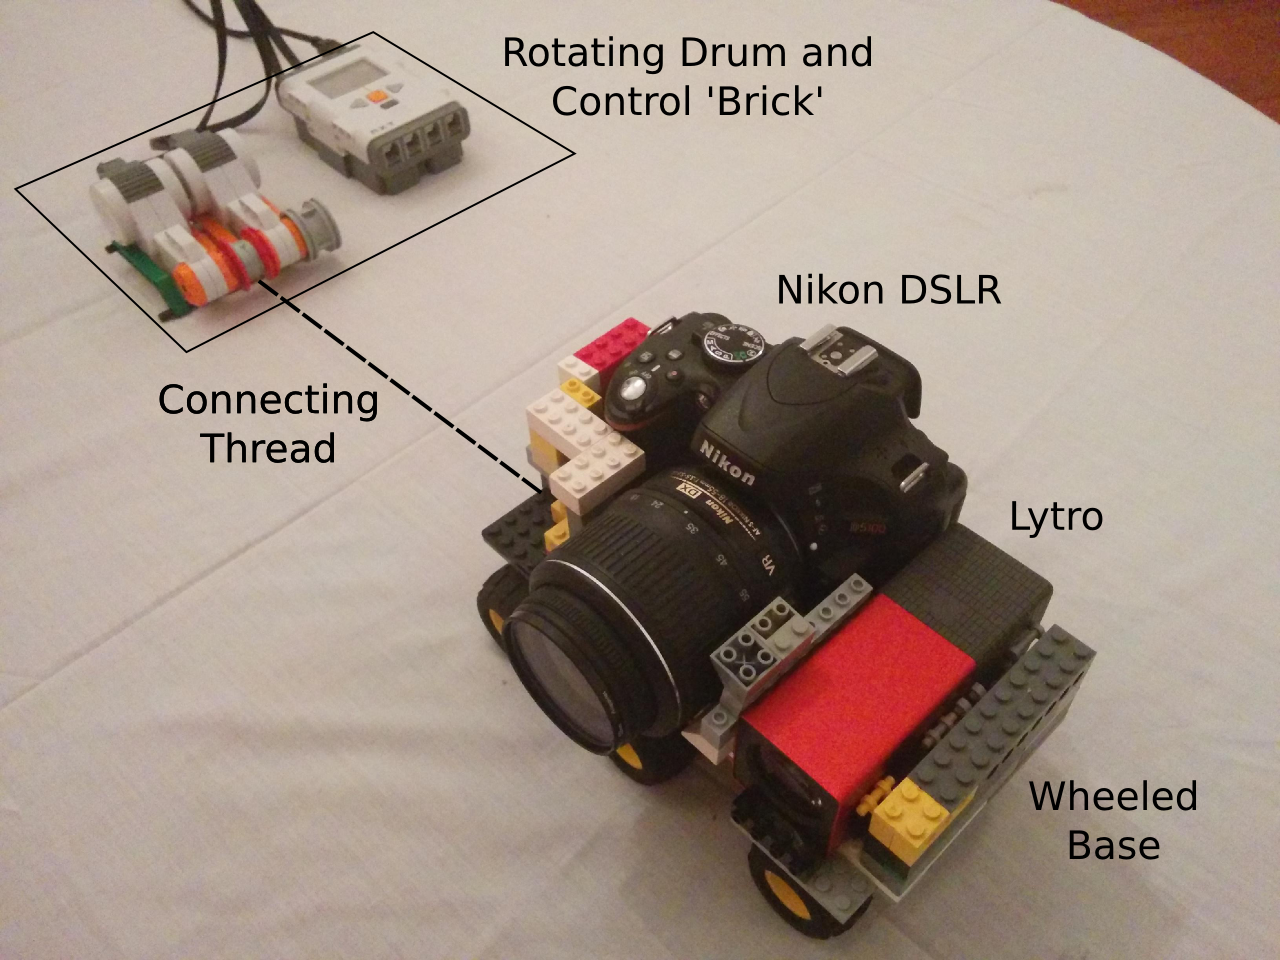
\includegraphics[width=\textwidth]{motion_platform}

\caption{Linear motion platform design}
\label{fig:motion_platform}

\end{figure}


\section{Scene Design}

The photographic scenes were set up in a room with no external facing windows to ensure the scene brightness could be controlled.
Three 60 watt incandescent ceiling light bulbs were used for ambient lighting and a single 72 watt diffuse incandescent desk lamp was used to provide extra light.
The desk lamp was arranged facing front-on to the scene to reduce shadow length and was placed behind the linear motion platform carrying the cameras.
A plain white sheet was placed on the working surface to reflect extra ambient light.

A large pin-board was placed behind the scene to provide a constant background depth and hardcover books were used to elevate scene elements where necessary.
Figure \ref{fig:scene_description} shows the experimental scene configuration.

\begin{figure}[h]

\centering

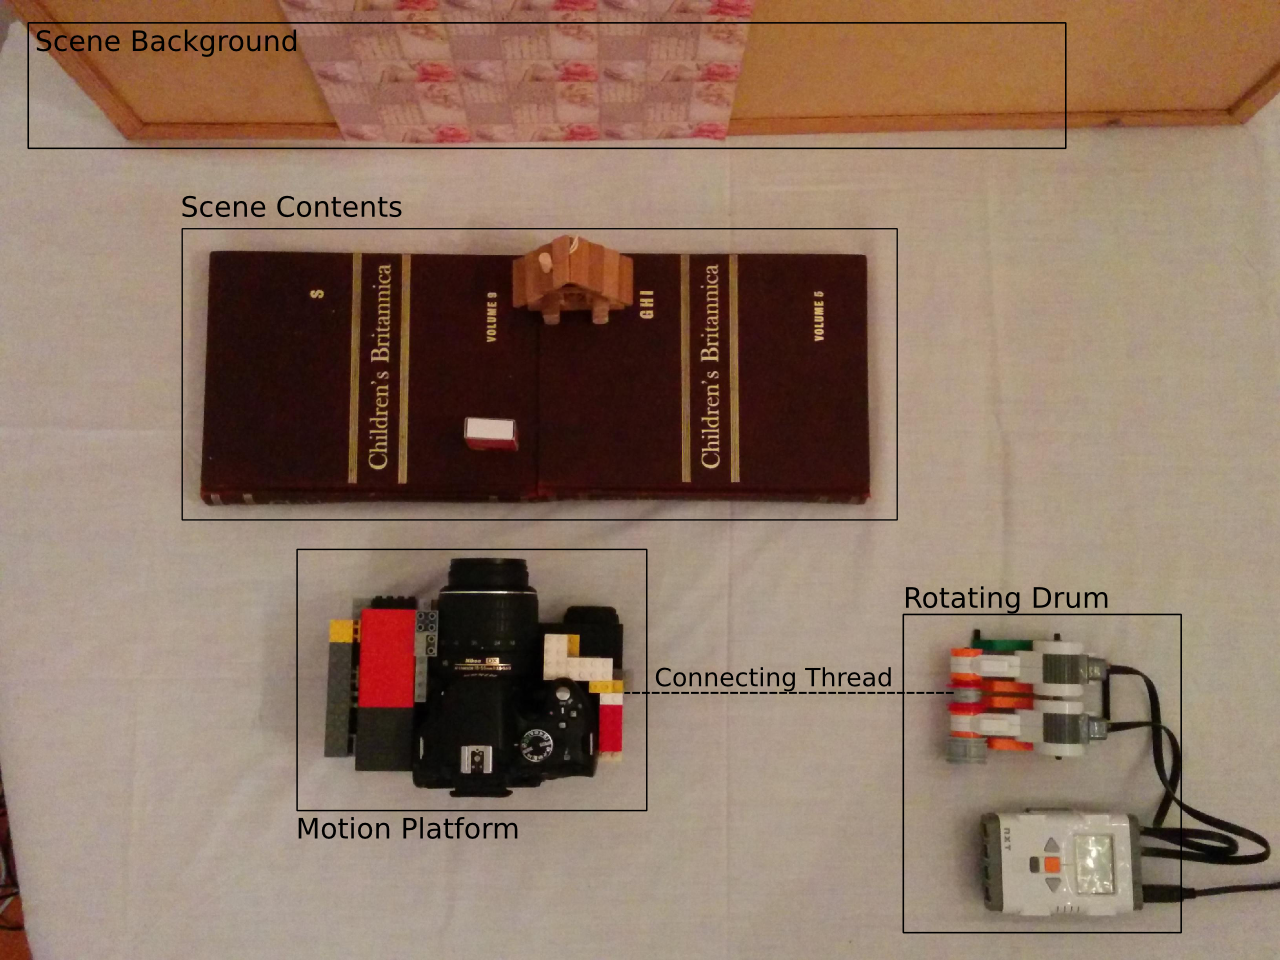
\includegraphics[width=\textwidth]{scene_contents}

\caption{Experimental scene layout, shown from above}
\label{fig:scene_description}

\end{figure}


\section{Image Capture}

A Lytro camera with firmware version 1.2.2 was used for the light field photography.
The Lytro camera was configured using the following settings.

\begin{table}[h]

\centering
\caption{Lytro Camera Settings}
\label{tab:lytro_settings}

\begin{tabular}{r | l}

Zoom & 1.0 \\
Creative Mode & Off \\
ND Filter & Off \\
ISO Sensitivity & Auto \\
Shutter Speed & As Required \\
Shutter Delay & 10s \\

\end{tabular}
\end{table}

The shutter delay was set to 10s to allow the motion platform to reach a stable velocity.
Once the camera countdown was started, the motion platform was commanded to move for a set distance at a set velocity.
In several cases multiple attempts were required to get the entire scene within the narrow Lytro field of view.

The captured images were transfered to an computer using the standard Lytro Desktop companion software, version 3.1.1 for Mac.
A late 2011 model Apple Mac Book Air running OSX 10.9.3 was used for image processing and version 0.2 of the Light Field Toolbox \cite{dansereau2013toolbox} was used for light field manipulation and processing in Matlab.
The image decoding, calibration and rectification process used by the LF toolbox is described in \cite{dansereau2013decoding}.

Lytro .lfp files were converted to raw image files and metadata files using the python-lfp-reader Python scripts (version 0.2) \cite{esfahbod2013python}, as per the Matlab LF Toolbox instructions.


\section{Image Processing and Deconvolution}

The raw image files were read using the Matlab LF Toolbox, and color correction applied.
The a-priori depth maps were read as images and the depth at several points in the depth map specified interactively using a graphical interface.

NEED TO TALK HERE ABOUT THE FACT THAT A-PRIORI CAMERA MOTION VELOCITY INFORMATION WAS USED, HOWEVER IN A REAL ENVIRONMENT OTHER SOURCES COULD BE USED TO GET THIS INFORMATION, E.G. THE BUILT-IN LYTRO ACCELEROMETER, OR A GPS OR OTHER SENSOR.

A least-squares regression was then performed to find a function mapping depth map intensity to real world depth.
To reduce processing time, the depth map was then posterized into a user-specified number of 'depth planes', each with a corresponding pixel mask.
The posterization was performed by applying 1-dimensional k-means clustering to the depth map histogram, using random seed locations.
A user-specified tolerance was used to terminate the k-means operation.
Figure XXXX shows the k-means clustering process.

[Figure XXXX goes here]

To de-blur the light field, all possible sup-aperture slices were taken and individually de-convoled once at every scene depth using the Richardson Lucy method, as implemented in the Matlab command 'deconvlucy'.
The de-convoled sub-aperture images were then combined, using the depth plane pixel masks.
This process is described in pseudocode in Listing XXXX.

[Listing XXXX goes here (pseudocode describing de-blurring)]


%LF_deblurred = new_empty_lf();
%
%for i = 1 to number_of_z_planes
%    blur_length = depth_map_to_blur_length(z_plane[i])
%    psf = make_motion_psf(blur_length);
%    
%    LF_deblurred_i = new_empty_lf();
%    
%    for j = 1 to microlens_width
%        for k = 1 to microlens_height
%            subap_image = LF_blurred(j, k, :, :, :)
%            deblurred = deblur_image(subap_image, psf)
%            LF_deblurred_i(j, k, :, :, :) = deblurred
%        end
%    end
%    
%    where z_plane[i] exists:
%        copy LF_deblurred_i pixels to LF_deblurred
%end


\section{Quantitative Analysis}

Two quantitative measures were used to compare de-blurred light fields.
A 'Q-Factor' was computed to measure the reduction in image blur and the Root-Mean-Square Error (RMSE) was estimated to measure the degree of noise amplification introduced by the de-convolution.

The Q-Factor was computed by taking the central sub-aperture image from the light field and using ImageJ to manually measure the blur width in pixels of prominent straight edges within the scene.
The same edges were measured in the blurred and de-blurred images, and '\% Q increase' calculated using

\begin{equation}
Q = \frac{1}{N} \sum_{i}^{N}(1 - \frac{w_{ai}}{w_{bi}}) * 100
\end{equation}

where $i$ refers to each edge measurement, and $w_{ai}$ and $w_{bi}$ are the edge widths in pixels after and before de-blurring respectively.

The RMSE was estimated by converting the central sub-aperture image to grayscale, then selecting a small (approximately 50x50 pixel) region known to be of constant color.
The RMSE was then computed using

\begin{equation}
R = \sqrt{ \sum_{x=1}^{W} \sum_{y=1}^{H} (I(x,y) - m)^2 }
\end{equation}

Where $W$ and $H$ are the width and height of the region respectively, $I$ is the region image and $m$ is the gray level within the region.



\chapter{Results}

Lots of results here.


\chapter{Discussion}

Limitations of study and results

Recap / discuss results

Implications of results

Further research and or extrapolation


\chapter{Conclusion}
\label{chap:conclusion}

Light field cameras are a revolutionary new form of imaging that enable many unconventional photographic techniques.
While these cameras have seen applications in a range of areas, their use in robotics has not yet been fully realised.
Unfortunately, some robotic navigation and computer vision systems suffer from the presence of motion blur in images.

State of the art deconvolution de-blurring techniques have the major drawback that they only work for scenes with a constant depth.
Robotic systems, especially ground or underwater mobile robots, typically operate in environments where the constant depth approximation is invalid.
For this reason, a means for de-blurring images at all scene depths is desirable.
Deriving a so-called \enquote*{depth-aware deonvolution} method was the focus of our research.

By analysing the math describing projective camera geometry an equation describing the formation of motion blur in a translating camera was derived (Equation \ref{eq:blur_width_simple}).
This equation was verified experimentally (Figure \ref{fig:blur_vs_depth}), indicating that calibrated depth data can be combined with camera intrinsic and trajectory information to perform depth-aware deconvolution.

It was found experimentally that Lytro depth maps can be calibrated to metric units using an empirically-determined piecewise linear mapping (Equation  \ref{eq:lytro_dm_to_metric}), provided a rough scene depth is known.

An experiment was performed to test the simplified case of linear camera motion blur at short distances.
Depth-aware deconvolution was compared with traditional de-blurring methods for three scenes using household objects.
The results showed that our method resulted in more high-frequency content and less ringing noise than 2D deconvolution methods.
It was found our method's performance was on-par with 2D deconvolution in scenes with little scene structure, due to the adverse effect this has on depth map estimation.

Our research made the assumption of linear camera motion, and relied on a rough scene depth estimate being supplied.
Additionally, our experiments were performed in a controlled environment.
Many areas for future work were identified, including adapting our method to generalised camera trajectories, utilising light field confidence information, collection of further data to confirm our results and the possibility of optimising our code to try and achieve real-time operation.
Perhaps the most interesting area to explore in the future is the possibility of using blind deconvolution methods to recover camera velocity whilst simultaneously de-blurring the light field.

Light field cameras have a host of potential applications in robotic systems.
It is hoped that our research and work demonstrating the feasibility of depth-aware deconvolution will enable further use of this exciting new technology.


\bibliographystyle{plain}
\bibliography{bibliography/thesis_bibliography}

\end{document}